\documentclass[10pt,a4paper, twocolumn, conference]{IEEEtran}
\author{Adam Lee}
\title{Multiple Linear Regression}
\date{November 2020}
\usepackage{amsthm}
\usepackage{pgfplots}
\usepackage{graphicx}
\usepackage{float}
\usepackage{amsmath}
\usepackage{amsfonts}
\usepackage{amssymb}
\usepackage{verbatim}
\usepackage{amsbsy}
\usepackage{algorithm}
\usepackage{algorithmic}
\usepackage[T1]{fontenc}
\usepackage[utf8]{inputenc}
\usepackage{hyperref}
\usepackage{cleveref}
\usepackage{placeins}
\usepackage{subcaption}
\usepackage{tablefootnote}
\DeclareMathOperator{\var}{var}
\renewcommand{\tabcolsep}{18pt}
\newtheoremstyle{own}%
    {5pt}% Space above
    {5pt}% Space below
    {}% Body font
    {}% Indent amount
    {\color{black}\bfseries}% Theorem head font
    {:}% Punctuation after theorem head
    {5pt}% Space after theorem head
    {}% Theorem head spec
\theoremstyle{own}
\newtheorem{example}{Example}
\theoremstyle{definition}
\newtheorem{definition}{Definition}
\theoremstyle{plain}
\newtheorem{thm}{Theorem}
\begin{document}
\maketitle
\pagebreak
\section{Introduction}
Our definition of linearity yields a significant amount of flexibility for our regression models. We can extend our definition for simple linear regression to form a regression model with multiple regressors each of which does not itself need to be linear but instead is accompanied by a linear coefficient. That is we can fit a model
\begin{equation} \label{eq1}
y = \beta_0 + \beta_1 x_1 + \cdots + \beta_n x_n + \varepsilon,
\end{equation}
where $y$ is our response variable and $x_i$ for $i = 1, \ldots, n$ are our regressors. It must be noted the term linear is used here since \cref{eq1} is a linear function of the unknown parameters $\beta_i$. This means we can choose our regressor terms freely. More complex models may allow for a polynomial fit.
\begin{example}
Consider the polynomial model
\begin{equation}
y = \beta_0 + \beta_1 x + \beta_2 x^2 + \varepsilon.
\end{equation}
If we let $x_i := x^i$ then this model takes the form
\begin{equation}
y = \beta_0 + \beta_1 x_1 + \beta_2 x_2 + \varepsilon,
\end{equation}
and is a linear regression model with three unknown regression coefficients and two regressors. It is still linear in our coefficients $\beta_i$ however allows a much more flexible model.
\end{example}

We can extend our definition of a multiple linear regression model further to include interaction terms. For example, consider the model
\begin{equation}
y = \beta_0 + \beta_1 x_1 + \beta_2 x_2 + \beta_{12} x_1 x_2.
\end{equation}
If we rewrite this model such that $\beta_{12} x_1 x_2 = \beta_3 x_3$ then we have a model of a familiar form
\[ y = \beta_0 + \beta_1 x_1 + \beta_2 x_2 + \beta_3 x_3.\]

\section{Multiple Linear Regression}
Let us focus on the generic case with model
\begin{equation}
y = \beta_0 + \beta_1 x_1 + \cdots + \beta_n x_n + \varepsilon.
\end{equation}

This model describes an $n + 1$ dimension hyperplane, as opposed to the regression line we constructed for the simple case. The parameters $\beta_i$ are our regression coefficients and in practice these, as well as the variance of the error $\epsilon$, are unknown. The particular parameter $\beta_j$ represents the expected change in $y$ per unit change in $x_j$ under the assumption that all other regressors $x_k,~( k \neq j )$ are constant. Figure \ref{fig1} provides graphic representation of a two-regressor, non-interacting model.
\vspace{2mm}
\hrule
\begin{example}
Consider a model where our expected error is zero
\begin{equation} \label{eq2}
E(y) = 10 + 15x_1 + 4x_2.
\end{equation}
We can examine the hyperplane this model describes.
\begin{figure}[H]
\centering
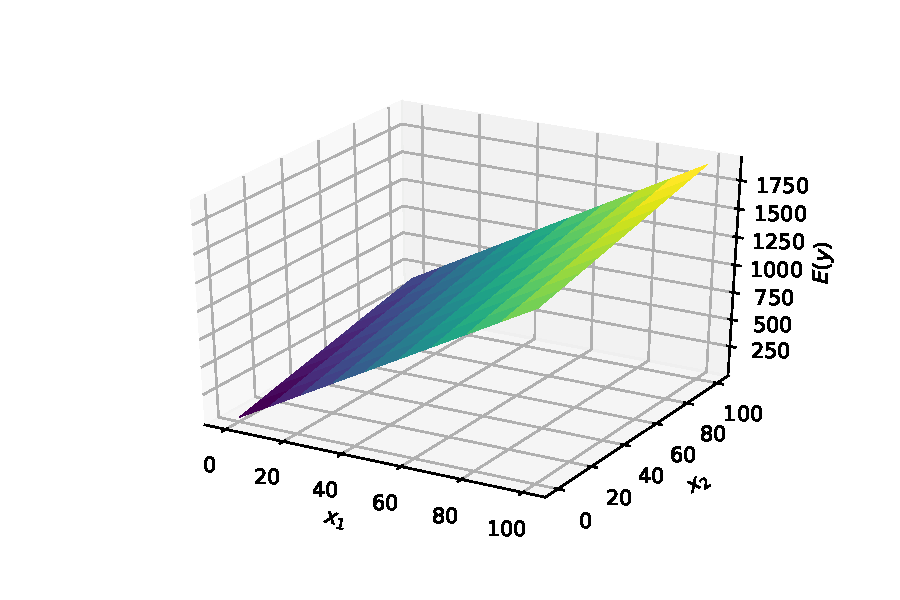
\includegraphics[width = 0.5\textwidth]{f4}
\caption{Hyperplane plot for \cref{eq2}}
\label{fig1}
\end{figure}
\end{example}
\hrule
\vspace{2mm}

Let us assume we have a data-set $\varkappa = \{y_i, x_{i1}, \ldots, x_{in} \}_{i=0}^k$ where $n > k$. Here, $y_i$ denotes the $i$-th observed response and $x_{ij}$ denotes the observed value $x_i$ for regressor $x_j$. Then, we have a system of model equations
\begin{equation}
y_i = \beta_0 + \beta_1 x_{i1} + \beta_2 x_{i2} + \cdots + \beta_n x_{in} ~~ i = 0, \ldots, k.
\end{equation}
We can then assume matrix notation for the entire set such that
\begin{equation}
\mathbf{y} = X \boldsymbol\beta + \boldsymbol\varepsilon.
\end{equation}
where
\begin{equation}
\mathbf{y} = \left( \begin{matrix} y_0 \\ y_1 \\ \vdots \\ y_k \end{matrix} \right),
\end{equation}
\begin{equation}
X = \left( \begin{matrix}
1 & x_{01} & \cdots & x_{0n} \\
1 & x_{11} & \cdots & x_{1n} \\
\vdots & \vdots & \ddots & \vdots \\
1 & x_{k1} & \cdots & x_{kn} 
\end{matrix} \right),
\end{equation}
\begin{equation}
\boldsymbol\beta = \left( \begin{matrix} \beta_0 \\ \beta_1 \\ \vdots \\ \beta_n \end{matrix} \right),
\end{equation}
and
\begin{equation}
\boldsymbol\varepsilon = \left( \begin{matrix} \varepsilon_0 \\ \varepsilon_1 \\ \vdots \\ \varepsilon_k \end{matrix} \right).
\end{equation}
The task then becomes fitting this linear model such that the coefficients $\boldsymbol\beta$ minimize the error term $\boldsymbol\varepsilon = \mathbf{y} - X \boldsymbol\beta$. A common method for determining these parameters is the method of least-squares, which we have already come across for the simple linear regression case. The same principles can be extended to multiple linear regression. Let us set $p = k+1, q = n+1$ moving forward for convenience.
\section{Method of Least-Squares}
Let us define the multivariate least-squares criterion function
\begin{align} \nonumber
\mathbb{E}(\boldsymbol\beta) := \sum_{i = 0}^k \varepsilon_i^2 & = \boldsymbol\varepsilon^{\text{T}} \boldsymbol\varepsilon = (\mathbf{y} - X \boldsymbol\beta)^{\text{T}} (\mathbf{y} - X \boldsymbol\beta) \\
& = \mathbf{y}^{\text{T}}\mathbf{y} - 2\boldsymbol\beta^{\text{T}}X^{\text{T}}\mathbf{y} + \boldsymbol\beta^{\text{T}}X^{\text{T}} X\boldsymbol\beta.
\end{align}
Then, we look for $k+1$ vector $\hat{\boldsymbol\beta}$ such that
\begin{equation}
\arg \min \mathbb{E} (\boldsymbol\beta) = \hat{\boldsymbol\beta}.
\end{equation}
To do so we must have
\begin{equation}
\frac{\partial \mathbb{E}}{\partial \boldsymbol\beta} \Big|_{\hat{\boldsymbol\beta}} = -2X^{\text{T}}\mathbf{y} + 2 X^{\text{T}} X \hat{\boldsymbol\beta} =  0,
\end{equation}
which we can simplify to
\begin{equation}
X^{\text{T}} X \hat{\boldsymbol\beta} = X^{\text{T}}\mathbf{y}.
\end{equation}
Then, provided the inverse matrix $(X^{\text{T}} X)^{-1}$ exists, our solution is
\begin{equation}
\hat{\boldsymbol\beta} = (X^{\text{T}} X)^{-1} X^{\text{T}}\mathbf{y}.
\end{equation}
Let us examine the matrix $X^{\text{T}} X$ in detail. By \cref{posdef}, $X^{\text{T}} X$ is a positive-definite matrix of the form
\begin{equation*} \arraycolsep=1.4pt\def\arraystretch{2.2}
\left[ \begin{array}{ccccc} q & \sum_{i = 0}^k x_{i1} & \sum_{i = 0}^k x_{i2} & \cdots & \sum_{i = 0}^k x_{in} \\
             \sum_{i = 0}^k x_{i1} & \sum_{i = 0}^k x_{i1}^2 & \sum_{i = 0}^k x_{i1}x_{i2} & \cdots & \sum_{i = 0}^k x_{i1}x_{in} \\
             \sum_{i = 0}^k x_{i2} & \vdots & \ddots & & \vdots\\
             \vdots				   & \vdots &  & \ddots & \vdots \\
             \sum_{i = 0}^k x_{in} & \sum_{i = 0}^k x_{i1}x_{in}  & \cdots & \cdots & \sum_{i = 0}^k x_{in}^2

\end{array} \right]
\end{equation*}
Inversion of this matrix can be tricky using orthodox methods in practical examples with large data-sets. However, we know enough about this matrix to manipulate it in such a way where this problem is simplified [\ref{ap:2}]. We can then test our parameters on some set of test points, say $\mathbf{x}^{*}$ then
\begin{equation}
\hat{\mathbf{y}} = \hat{X} \hat{\boldsymbol\beta} = \hat{X} (X^{\text{T}} X)^{-1} X^{\text{T}}\mathbf{y} = H\textbf{y},
\end{equation}
where $\hat{X}$ is the corresponding $X$ for the test points $\mathbf{x}^{*}$. We call the matrix $H$ the hat matrix of our model, since it puts a hat on $\mathbf{y}$


\appendix
\section{Linear Algebra Proofs}
\begin{thm} \label{posdef}
For any real, invertible matrix $A \in \mathbb{R}^{n \times n}$, the product matrix $A^{\text{T}}A$ is positive definite i.e
\begin{equation}
\mathbf{z}^{\text{T}} A^{\text{T}}A \mathbf{z} > 0 ~ \forall ~ \mathbf{z} \in \mathbb{R}^{n}
\end{equation}
\end{thm}
\begin{proof}
\begin{align} \nonumber
\mathbf{z}^{\text{T}} A^{\text{T}}A \mathbf{z} & = (A \mathbf{z})^{\text{T}} (A \mathbf{z}) \\
& = || Az ||^2 > 0.
\end{align}
\end{proof}
\begin{thm} \label{ap:2}
For a positive-definite matrix $A$, there exists a lower-triangular matrix $U$ such that
\begin{equation}
A^{-1} = U U^{T}
\end{equation}
\end{thm}
\begin{proof}
For positive-definite matrix $A$, we have a Cholesky decomposition such that
\begin{equation}
A = L L^{\text{T}},
\end{equation}
then we have
\begin{equation}
A A^{-1} = L L^{\text{T}} A^{-1} = I,
\end{equation}
that is
\begin{equation}
A^{-1} = ( L^{\text{T}} )^{-1} L^{-1}.
\end{equation}
Since $L$ is lower triangular, if we write $( L^{\text{T}} )^{-1} = U$ then we have
\begin{equation}
A^{-1} = U U^{\text{T}},
\end{equation}
which is a positive-definite symmetric matrix such that we need only compute the upper-triangular elements of $U U^{\text{T}}$ in order to know all elements of $A^{-1}$.
\end{proof}













 
\end{document}
